% !TEX root = ./notes.tex
\chapter{Plasma Physics}

Under the conditions in a stellar interior, most of the atoms are ionized, and the stellar matter consists of positively charged nuclei and ions and negatively charged electrons. More precisely,
a \emph{plamsa} is defined as a gas of charged particles in which the kinetic energy of a typical particle is much greater than the potential energy due to its nearest neighbors. To make this quantitative, consider a gas with only one species present, with charge $q$.  Let the mean spacing between particles be $a$; clearly the number density of such particles is $n = (4\pi a^{3}/3)^{-1}$.  We may then take the quantity
\begin{equation}\label{e.Gamma-definition}
\Gamma \equiv \frac{q^{2}}{a\kB T}
\end{equation}
as indicating the relative importance of potential to kinetic energy.  In a classical plasma, $\Gamma \ll 1$.  Note, however, that systems with $\Gamma > 1$ are often (confusingly) called  \emph{strongly coupled plasmas}. The meaning is usually clear from context.

\section{Debye shielding}\label{s.plasma-shielding}

Imagine a typical charged particle in a plasma.  Very close to the particle, we expect the electrostatic potential to be that of an isolated charge $\Phi = q/r$. Far from the particle, there will be many other particles surrounding it, and we may expect that the potential to be screened. For example, a positive ion will tend to attract electrons to be somewhat closer, on average to it: we say that the ion \emph{polarizes} the plasma.  As a result of this polarization, the potential of any particular ion should go to zero much faster than $1/r$ due to the ``screening'' from the enhanced density of opposite charges around it.

Let's consider a plasma having many ion species, each with charge $Z_{i}$, and elections. About any selected ion $j$,  particles will arrange themselves according to Boltzmann's law,
\begin{equation}\label{e.ion-boltzmann}
n_{i}(r) = n_{i0}\exp\left[-\frac{Z_{i}e\Phi(r)}{\kB T}\right].
\end{equation}
Here $n_{i0}$ is the density of particle $i$ far from the charge $j$, and $r$ is the distance between particles $i$ and $j$.  (A similar equation holds for the electrons, with $Z$ replaced by $-1$.) To solve for the potential, we can use Poisson's equation,
\begin{equation}\label{e.Poisson}
\nabla^{2}\Phi = -4\pi \sum_{i} Z_{i}e n_{i}(r) +4\pi e n_{e}(r).
\end{equation}
Our assumption is that the term in the exponential of equation~(\ref{e.ion-boltzmann}) is small, so we may expand it to first order in $\Phi$ and substitute that expansion into equation~(\ref{e.Poisson}) to obtain in spherical geometry
\[
 \frac{1}{r}\frac{\partial^{2}}{\partial r^{2}}\left(r\Phi\right) = -4\pi e \left[\sum_{i} n_{i0}Z_{i}\left(1-\frac{Z_{i}e\Phi}{\kB T}\right) - n_{e0}\left(1 + \frac{e\Phi}{\kB T}\right)\right].
\]
The overall charge neutrality of the plasma implies that $n_{e0} = \sum_{i}Z_{i}n_{i0}$; using this to simplify the above equation gives
\begin{equation}\label{e.linearized-Poisson}
\frac{1}{r}\frac{\partial^{2}}{\partial r^{2}}\left(r\Phi\right) = \left[\frac{4\pi e^{2}}{\kB T}\sum_{i} n_{i0}\left(Z_{i}^{2}+Z_{i}\right)\right]\Phi \equiv \lambdaD^{-2}\Phi.
\end{equation}
The quantity in $[\, ]$ has dimensions of reciprocal length squared and we define it as $(1/\lambdaD)^{2}$ with $\lambdaD$ being called the \emph{Debye length}.

Multiplying equation~(\ref{e.linearized-Poisson}) by $r$, integrating twice, and determining the constant from the condition that as $r\to 0$, $\Phi \to Z_{j}e/r$ gives the self-consistent potential
\begin{equation}\label{e.screened-potential}
\Phi = \frac{Z_{j}e}{r}\exp\left(-\frac{r}{\lambdaD}\right).
\end{equation}
The Debye length \lambdaD\ determines the size of the screening cloud around the ion.

In order for the above derivation to be valid, we require that $\lambdaD \gg a$, where $a$ is the mean ion spacing; otherwise, there won't be any charges in our cloud to screen the potential! Equivalently, we require the number of particles in a sphere of radius \lambdaD\ to be large,
\begin{equation}\label{e.plasma-parameter}
\frac{4\pi}{3}\lambdaD^{3} \sum_{i} n_{i} \gg 1.
\end{equation}
This condition must hold if we are to treat the gas as a plasma.

\section{Corrections to the ideal gas EOS}\label{s.plasma-corrections}

In a plasma the particles are not independent: shake one particle and other nearby particles will shake as well. In statistical mechanics, this requires introducing \emph{correlation functions} to derive the equation of state.  We'll adopt the more intuitive approach of Debye and H\"uckel to get the lowest-order correction to the ideal gas EOS.  First, the total electrostatic energy in a volume $V$ is
\begin{equation}\label{e.electrostatic-energy}
E_{\mathrm{Coul}} = \frac{1}{2}V\sum_{j}Z_{j}e n_{j}\Phi_{j}.
\end{equation}
Here $\Phi_{i}$ is the potential at a particle $j$ \emph{due to all the other particles in the plasma.}  Now, we computed the total potential around a particle (eq.~[\ref{e.screened-potential}]); expanding and subtracting off the self-potential of particle $j$ gives $\Phi_{j} = -Z_{j}e/\lambdaD$.  Inserting this into equation~(\ref{e.electrostatic-energy}) and expanding gives
\begin{equation}\label{e.electrostatic-energy-2}
E_{\mathrm{Coul}} \approx - V\left(\frac{\pi}{\kB T}\right)^{1/2} e^{3} \left[\sum_{i}n_{i0} \left(Z_{i}^{2} + Z_{i}\right)\right]^{3/2}.
\end{equation}
This energy is to be added to the kinetic energy of the gas.  The effect of the electrostatic interactions is to \emph{decrease} the energy in the gas, that is, to make it more bound.

In order to get the pressure, we first must find the Helmholtz free energy $A$ (we can't directly differentiate equation~[\ref{e.electrostatic-energy-2}] because it isn't in terms of $S$ and $V$). Integrating the thermodynamical identity $E = -T^{2}(\partial/\partial T)(A/T)$ and then taking $P = -(\partial A/\partial V)_{T,N}$ gives
\begin{equation}\label{e.pressure-correction}
 P_{\mathrm{Coul}} \approx -\frac{e^{3}}{3}\left(\frac{\pi}{\kB T}\right)^{1/2}\left[\frac{\left(\langle Z^{2}\rangle+\langle Z\rangle \right)\rho}{\langle A\rangle\mb}\right]^{3/2}.
\end{equation}
The effect of Coulomb interactions is to decrease the pressure below the ideal gas value.

\section[Strongly Coupled Plasmas]{Coulomb corrections when the electrons are degenerate}\label{s.degenerate-coulomb}

The above discussion holds only when both the electrons and ions are non-degenerate.  What happens when the electrons are degenerate?  In that case the kinetic energy is of order the Fermi energy, not the temperature.  We might think to replace $\kB T$ with \eF\ in equation~(\ref{e.Gamma-definition}). Recalling the formula for \eF\ from \S~\ref{s.deg-limit-fermions}, we have the condition for weak interactions,
\begin{equation}\label{e.condition-weak-degen}
\frac{e^{2}}{a \eF} = \left(\frac{4\pi n}{3}\right)^{1/3}\left(\frac{m_{e} e^{2}}{\hbar^{2}}\right)\frac{2}{(3\pi^{2} n)^{2/3}} < 1.
\end{equation}
Here $m_{e}$ and $n$ denote, respectively, the electron mass and number density.  Do you recognize the quantity $\hbar^{2}/(m_{e}e^{2})$?  It is the Bohr radius, \abohr.  What is \abohr\ doing in this equation?  Well, we are looking for a quantum mechanical system in which the Coulomb interaction is comparable to the non-relativistic kinetic energy.  Does that sound like any system you've seen before?

Cleaning up equation~(\ref{e.condition-weak-degen}), our condition for the electrons to be weakly interacting when degenerate is
\begin{equation}
\left(\frac{2^{5/3}}{3\pi}\right)\left( n \abohr^{3}\right)^{-1/3} < 1,
\end{equation}
or, in terms of mass density $\rho$ and electron fraction $Y_{e}$, $(Y_{e}\rho) > 0.4\nsp\grampercc$.  As the density increases, the electron gas becomes more ideal, that is, the electrostatic interaction matters less and less.  

Just to complete the discussion on electrons, what if the electrons are relativistic?  In this case, $\eF = \pF c = (3\pi^{2}n)^{1/3}\hbar c$, and
\begin{equation}\label{e.condition-weak-rel-degen}
\frac{e^{2}}{a \eF} = \left(\frac{4}{9\pi}\right)^{1/3}\left(\frac{e^{2}}{\hbar c}\right) = 3.8\ee{-3}.
\end{equation}
In this case $\eF \propto n^{1/3}$ so the density dependence cancels.  You will note the appearance of the fine structure constant $\alpha_{\mathrm{F}} = e^{2}/(\hbar c)$, as you might have expected when dealing with relativistic electrons and electrostatics.

Under astrophysical conditions, we can almost always regard degenerate electrons as being ideal.  What about the ions?  They are not usually degenerate under conditions of interest. We can get a simple expression if we go to the opposite limit, in which the electrons are very degenerate.  In that case, the electrons are an ideal gas and hence have uniform density. If the temperature is low enough, the ions will have $Z^{2}e^{2}/(a\kB T) \gg 1$; in this case we might expect the ions will arrange themselves into a lattice that maximizes the inter-ionic spacing.

To get an estimate of the electrostatic energy, let's compute the energy of a charge-neutral sphere centered on a particular ion of charge $Z_{i}$.  Because the electrons have a uniform density, $Y_{e}\rho/\mb$, we can find the radius of the sphere $a$ by requiring it to have $Z_{i}$ electrons,
\begin{equation}\label{e.radius-ion-sphere}
\frac{4\pi}{3}a^{3}\left(Y_{e}\frac{\rho}{\mb}\right) = Z_{i},
\end{equation}
or $a = [3 Z_{i} \mb/(4\pi Y_{e}\rho)]^{1/3}$.  The potential energy of this sphere has two components. The first is due to electron-electron interactions,
\begin{equation}\label{e.ee-energy}
E_{ee} = \int_{0}^{a} \frac{q(r)\, \dif q}{r} = \frac{3}{5}\frac{Z_{i}^{2}e^{2}}{a},
\end{equation}
where $q(a) = Z_{i}e(r/a)^{3}$ is the charge in a sphere of radius $r < a$. The second component of the potential energy is due to the ion-electron interaction,
\begin{equation}\label{e.ei-energy}
E_{ei} = -Z_{i}e\int_{0}^{a}\frac{\dif q}{r} = -\frac{3}{2}\frac{Z_{i}^{2}e^{2}}{a}.
\end{equation}
Combining equations~(\ref{e.ee-energy}), (\ref{e.ei-energy}), and (\ref{e.radius-ion-sphere}) gives the total electrostatic energy for a single ion-sphere,
\begin{equation}\label{e.madelung-sphere}
E = -\frac{9}{10} \frac{Z_{i}^{2}e^{2}}{a} = -\frac{9}{10} Z_{i}^{5/3} e^{2} \left(\frac{4\pi}{3}\frac{Y_{e}\rho}{\mb}\right)^{1/3}.
\end{equation}
Multiplying this by $n_{i} = Y_{i}\rho/\mb$, summing over all ion species $i$, and defining $\langle Z^{5/3}\rangle = n^{-1}\sum Z_{i}^{5/3}n_{i}$ where $n = \sum n_{i}$, gives the total Coulomb energy per volume,
\begin{equation}\label{e.madelung-total}
E_{\mathrm{Coul}} = -\frac{9}{10} n\kB T \left[\frac{\langle Z^{5/3}\rangle e^{2}}{\kB T}\left(\frac{4\pi}{3}\frac{Y_{e} \rho}{\mb}\right)^{1/3}\right].
\end{equation}
Notice that the quantity in $[\nsp]$ reduces to $\Gamma$ for a single-species plasma.  If we therefore define $\Gamma \equiv [\nsp]$ for a multi-component plasma, we have $E_{\mathrm{Coul}} \approx -0.9 n\kB T \Gamma$; the pressure is then $P_{\mathrm{Coul}} = E_{\mathrm{Coul}}/3  = -0.3 n \kB T \Gamma$. This holds in the limit $\Gamma \gg 1$.

\section{Collisions}\label{s.plasma-collisions}

Without collisions, a plasma cannot reach thermodynamic equilibrium, and the rate of collisions mediates both the approach to equilibrium and the transport of quantities, such as heat, in a forced system. In this section, we'll make an estimate for the rate of electron-electron ion-ion, and electron-ion collisions.

To begin, let's imagine a light particle (electron) colliding with a much heavier, fixed particle (an ion), as illustrated in Figure~\ref{f.scattering}.  (This picture also applies to a pseudo particle of reduced mass scattering in a fixed potential.)  Let the impact parameter be $b$, and the mass of the incident particle is $\mu$.  For Coulomb interactions, the force on the particle is $(q_{1}q_{2}/r^{2})\bvec{\hat{r}}$. The incident momentum is $p_{0}$. Now by assumption, in our plasma most of the interactions are weak (potential energy is much less than kinetic), so let's treat the deflection of the particle as a perturbation.  That is, we shall assume that $p_{0} = \textrm{const}$ and that the effect of the interaction is to produce a perpendicular (to $p_{0}$) component of the momentum $p_{\bot}$.  The total change in $p_{\bot}$ is then
\[ p_{\bot} = \int_{-\infty}^{\infty}\dif t\; \frac{q_{1}q_{2}}{r^{2}}\sin\theta, \]
where $\sin\theta = b/r$ is the angle that the radial vector makes with the horizontal.  Substituting $r = b/\sin\theta$ and $\dif t = -\mu b \dif \theta/p_{0}/\sin^{2}\theta$, we have
\[ p_{\bot} = -\int_{0}^{\pi} \sin\theta\,\dif\theta\; \frac{\mu}{p_{0}}\frac{q_{1}q_{2}}{b}, \]
leading to the intuitive result
\begin{equation}\label{e.pperp}
\frac{p_{0}p_{\bot}}{2\mu} = \frac{q_{1}q_{2}}{b}.
\end{equation}
Clearly a large angle scattering occurs if $p_{\bot}\ge p_{0}$, or
\begin{equation}\label{e.b0}
b \le b_{0} \equiv \frac{2\mu q_{1}q_{2}}{p_{0}^{2}};
\end{equation}
our approach is only valid for $b \gg b_{0}$.  Note that $p_{\bot}/p_{0} = b_{0}/b$. What is the rate of large angle  scatterings? The cross section for a large angle scattering is
$ \sigma_{\mathrm{LA}} = \pi b_{0}^{2}$.  Imagine a particle incident on a volume of particles.  imagine a cylinder of length $(p_{0}/\mu)\dif t \mathcal{A}$, where $\mathcal{A}$ is the cross-section of the cylinder.  Within this cylinder there are $n\times (p_{0}/\mu)\dif t \mathcal{A}$ scatterers of cross-section $\sigma_{\mathrm{LA}}$. so the probability of the particle interacting per time $\dif t$ is
\[ \frac{(\sigma_{\mathrm{LA}}\times n\times p_{0}/\mu) \mathcal{A}}{\mathcal{A}}  = n\sigma_{\mathrm{LA}} p_{0}/\mu. \]
This defines the large-angle collision rate,
\begin{equation}\label{e.large-angle-collision-rate}
\nu_{\mathrm{LA}} = n\sigma_{\mathrm{LA}} v_{0} = \frac{4\pi \mu (q_{1}q_{2})^{2}}{p_{0}^{3}}.
\end{equation}
Note that it goes as $p_{0}^{-3}$; fast-moving particles are hard to scatter.

\begin{figure}[htbp]
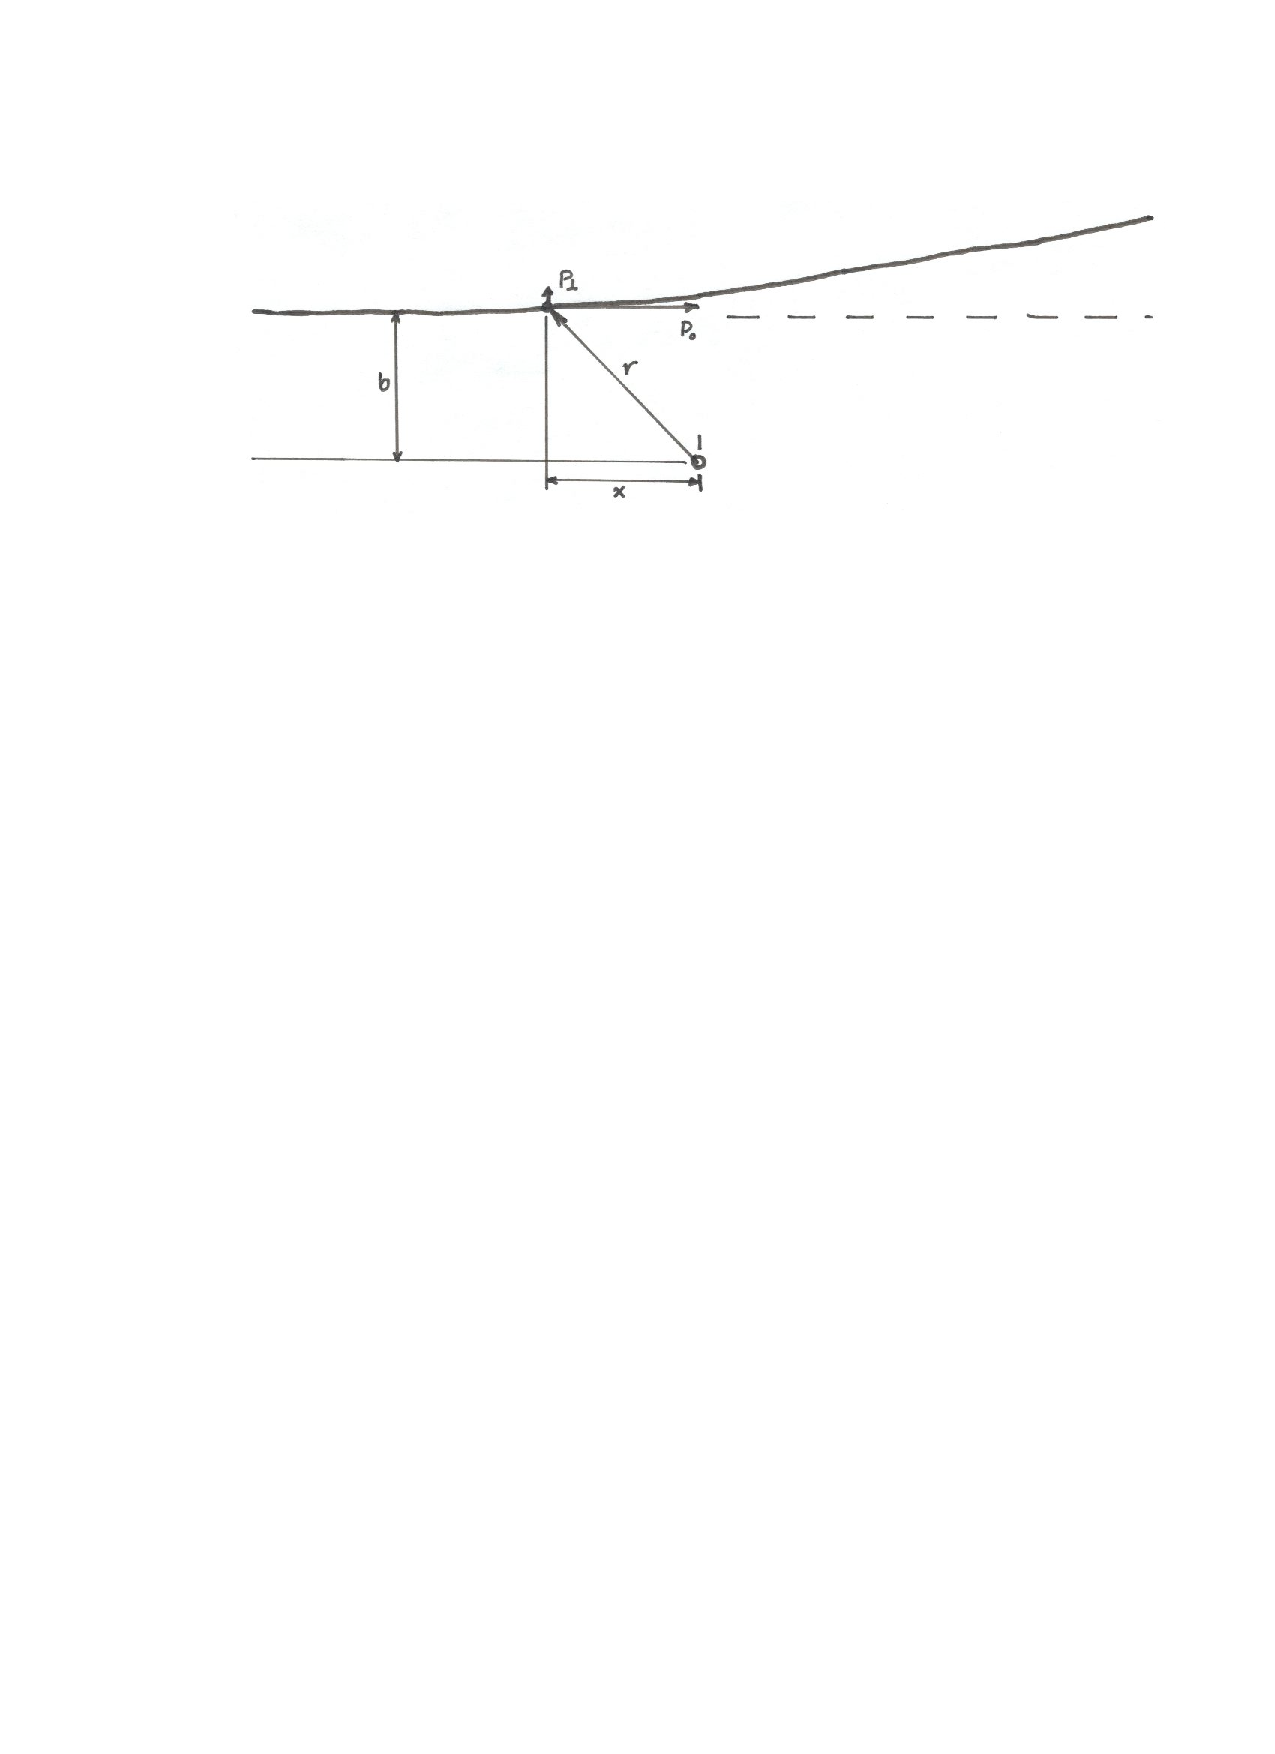
\includegraphics[width=\textwidth]{scattering}
\caption{Geometry for scattering problem.}
\label{f.scattering}
\end{figure}

As mentioned earlier, we are in a weakly coupled plasma, so we expect large angle scatterings to be a rare occurrence. What happens instead is that the particle suffers a number of small deflections. Let's consider an impact parameter in the range $(b,b+\dif b)$. Each deflection will have $\bvec{\Delta p}_{\bot}$ in some random direction, so
\[ \langle \bvec{ p}_{\bot}\rangle = \sum_{i=1}^{N} \bvec{\Delta p}_{i} \approx \bvec{0}. \]
What is happening is that the component of momentum perpendicular to $p_{0}$ is executing a random walk.  Indeed, after $N$ collisions,
\begin{eqnarray*} \langle \bvec{p}_{\bot} \vdot \bvec{p}_{\bot} \rangle  &=& \left( \sum_{i=1}^{N} \bvec{\Delta p}_{i}\right)\vdot \left( \sum_{i=1}^{N} \bvec{\Delta p}_{i} \right) \\
&=& \sum_{i=1}^{N} (\Delta p_{i})^{2} + 2\sum_{i\ne j} \bvec{\Delta p}_{i}\vdot\bvec{\Delta p}_{j} = N(\Delta p_{\bot})^{2},
\end{eqnarray*}
where we have assumed that all $\bvec{\Delta p}_{\perp}$ have the same magnitude and are uncorrelated. Now $N$ is just $\Delta t \times n \times (2\pi b \,\dif b) \times (p_{0}/\mu)$: the number of particles with impact parameters between $b$ and $b+\dif b$ along the length of the particles path over a time $\Delta t$.  Dividing by $\Delta t$ and integrating over $b$, we have the rate of change of the perpendicular component of the momentum
\begin{equation}\label{e.msdev-momentum}
\frac{\dif \langle p_{\bot}^{2}\rangle }{\dif t} = \frac{8\pi n\mu (q_{1}q_{2})^{2}}{p_{0}^{3}}\int_{b_{\mathrm{min}}}^{b_{\mathrm{max}}}\;\frac{\dif b}{b}.
\end{equation}
What are $b_{\mathrm{max}}$ and $b_{\mathrm{min}}$, the maximum and minimum impact parameters? Clearly, if $b > \lambda_{\mathrm{D}}$ then the potential will be screened.  Since our approximation is only good for $b > b_{0}$, we may take $b_{\mathrm{min}} = b_{0}$. (Our rate of scattering only depends logarithmically on $b_{\mathrm{max}}/b_{\mathrm{min}}$, so these estimates are good enough for our purposes).  With this substitution,
\begin{eqnarray}
\frac{\dif \langle p_{\bot}^{2}\rangle }{\dif t} &=& \frac{8\pi n\mu (q_{1}q_{2})^{2}}{p_{0}^{3}}\ln\left(\frac{\lambda_{\mathrm{D}}}{b_{0}}\right)\nonumber \\
 &\equiv& \frac{8\pi n\mu (q_{1}q_{2})^{2}}{p_{0}^{3}}\ln\Lambda.
\label{e.deflection-rate}
\end{eqnarray}
In the literature, the quantity $\ln\Lambda$ is called the Coulomb logarithm; for a plasma such as we are considering it is $\sim \ln  \left(\Lambda_{\mathrm{D}}^{3} n\right)$, the logarithm of the number of particles in a Debye sphere (see eq.~[\ref{e.plasma-parameter}]).  For conditions typical of the solar center (hydrogen plasma, $\rho \gtrsim 1\nsp\grampercc$, $T \approx 10^{7}\nsp\K$), $\ln\Lambda \approx \left(5\textrm{--}10\right)$.  

For small-angle scattering, the concept of a collision rate is fuzzy: the particle is constantly being bombarded by many tiny collisions.  Setting $\dif \langle p_{\bot}^{2}\rangle/\dif t = p_{0}^{2}$ allows us to define a deflection rate,
\begin{eqnarray}\label{e.scattering-rate}
\nu &\approx& \frac{8\pi n \mu (q_{1}q_{2})^{2}}{p_{0}^{3}} \ln\Lambda\\
 &=& \frac{8\pi n (q_{1}q_{2})^{2}}{(3\kB T)^{3/2}\mu^{1/2}}\ln\Lambda.
\end{eqnarray}
Comparing equations~(\ref{e.scattering-rate}) and (\ref{e.large-angle-collision-rate}), we see that many small angle scatterings are more important than single large angle scattering. Note that the ion-ion collision rate will be about $\sqrt{m_{p}/m_{e}} \approx 43$ times less than the electron-electron collision rate for a given temperature.

One can define a mean free path $\ell$ from equation~(\ref{e.scattering-rate}). Consider a particle incident on a cylinder of cross-sectional area $\mathcal{A}$ and length $\ell$, as illustrated in Figure~\ref{f.mfp}. We chose $\ell$ so that the time for the particle to traverse it is $\nu^{-1}$, the timescale for deflection.  Thus $\ell = v_{0}/\nu = p_{0}/(\mu\nu)$. Note that for a large angle collision, we can write the probability for scattering as the total cross-section of scatterers per unit area,
\begin{equation}\label{e.mfp-simple}
\mathcal{P} = \frac{N\sigma}{\mathcal{A}} = \frac{n\times(\ell\mathcal{A})\sigma}{\mathcal{A}},
\end{equation}
so the particle will suffer on average a collision after traversing a distance $\ell = (n\sigma)^{-1}$. Comparing equation~(\ref{e.mfp-simple}) with our expression for $\ell$ in terms of $\nu$ allows us to define an effective cross-section for small angle scattering.

\begin{figure}[htbp]
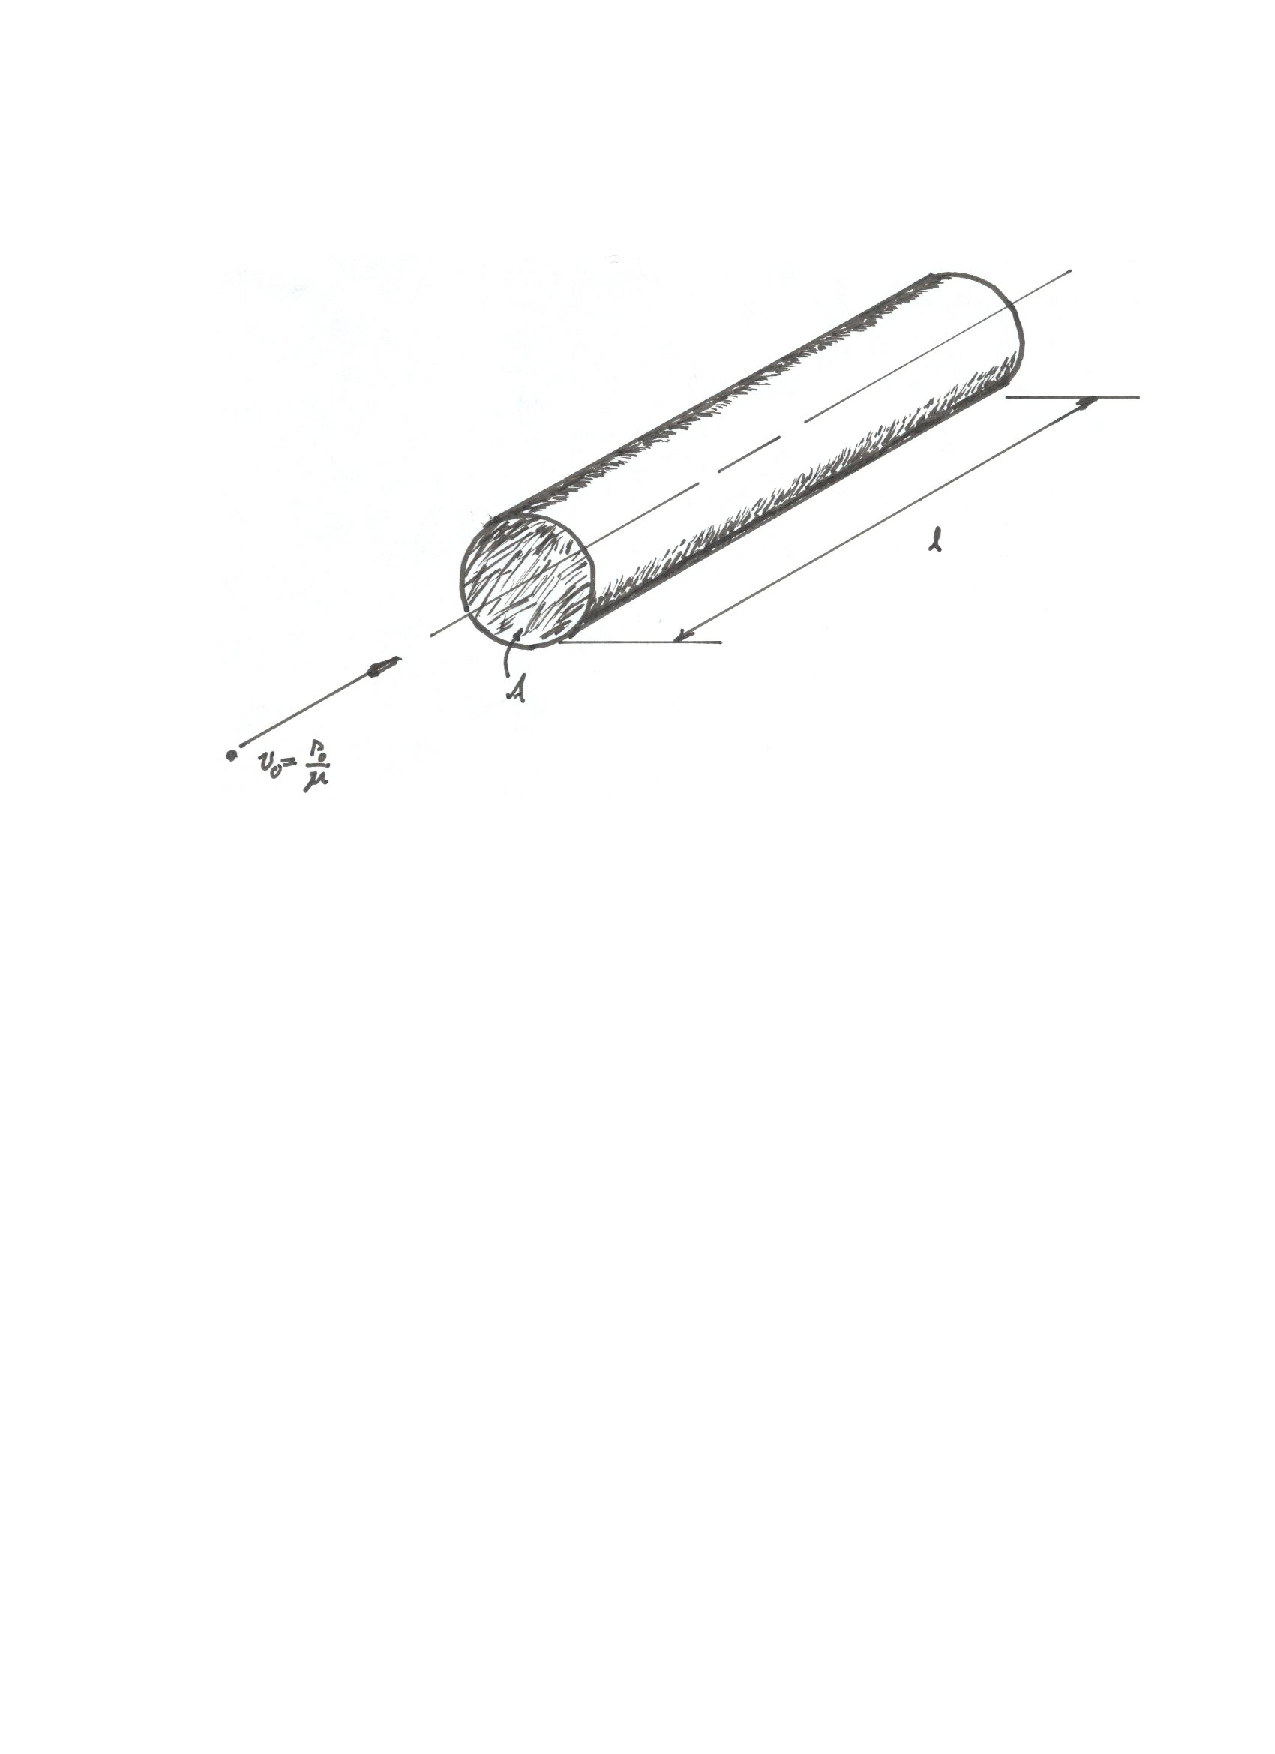
\includegraphics[width=\textwidth]{mean-free-path}
\caption{Schematic of a particle incident on a cylinder containing $n\times\ell\times\mathcal{A}$ particles.}
\label{f.mfp}
\end{figure}

\section{Transport properties}

We now have enough machinery to make estimates of \emph{transport coefficients,} such as the viscosity and the thermal conductivity. Let's begin with the viscosity.  Suppose we have a fluid with a gradient in the velocity, a shear, as depicted in Figure~\ref{f.shear-diagram}.  Let the mean thermal velocity of a particle be $v_{0}$.  In a time $\Delta t$, a number of particles will enter the box from the top, $(1/6) n v_{0} \Delta t$, and a similar number will leave the box via the top face. On average, these particles are endowed with the fluid properties of their last scattering, so the \emph{net} momentum carried into the box across the top face is
\begin{equation}\label{e.viscosity-1}
 \frac{1}{6} n m v_{0} \Delta t \Delta A \left[v_{y}(z_{t} + \ell) - v_{y}(z_{t}-\ell)\right] \approx \frac{1}{3} n m v_{0} \Delta t\Delta A \left.\frac{\partial v_{y}}{\partial z}\right|_{z_{t}}\ell.
\end{equation}
Here $\Delta A$ is the cross-section area of our box in the $xy$ plane and $z_{t}$ is the coordinate of the top face.

\begin{figure}[htbp]
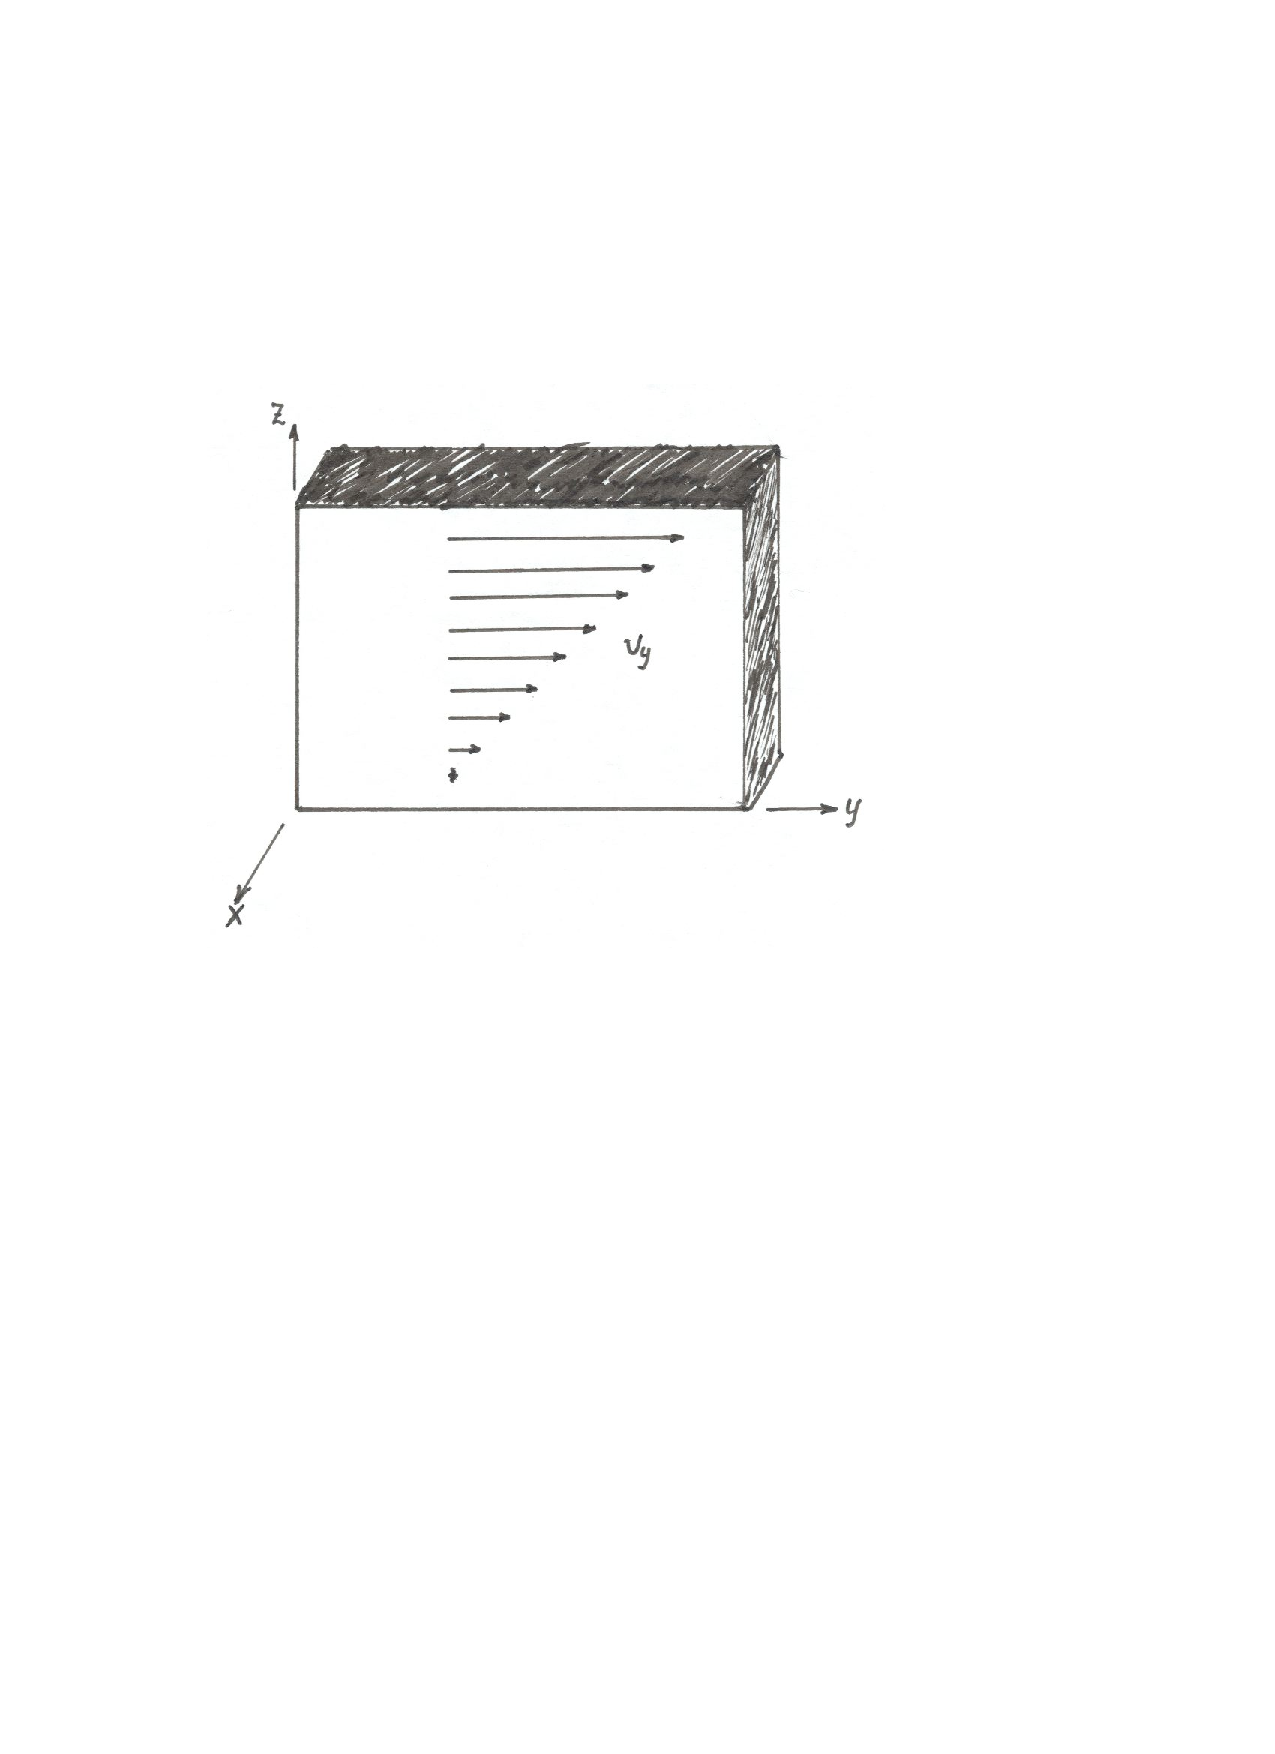
\includegraphics[width=\textwidth]{shear-diagram}
\caption{An element of fluid with a shear $\partial v_{y}/\partial z$.}\label{f.shear-diagram}
\end{figure}

A similar process occurs across the bottom face, located at coordinate $z=z_{b}$: the momentum flux across the bottom face is
\begin{equation}\label{e.viscosity-2} 
\approx -\frac{1}{3} n m v_{0} \Delta t\Delta A \left.\frac{\partial v_{y}}{\partial z}\right|_{z_{b}}\ell.
\end{equation}
Note the difference in sign: the momentum flux is positive if the $y$-velocity is larger below the box.  Putting equations~(\ref{e.viscosity-1}) and (\ref{e.viscosity-2}) together, the net change of momentum per time per unit volume $\Delta A\Delta z$ is
\begin{eqnarray}
\frac{1}{\Delta A\Delta z}\frac{\Delta p}{\Delta t} &\approx&  \frac{1}{\Delta z} \frac{1}{3} \left[\left(n m v_{0}\ell\frac{\partial v_{y}}{\partial z}\right)_{z_{t}} - \left(n m v_{0} \ell\frac{\partial v_{y}}{\partial z}\right)_{z_{b}}\right]\nonumber\\
 &\approx&   \frac{\partial}{\partial z}\left( \mu \frac{\partial v_{y}}{\partial z}\right).
\label{e.viscosity-3}
\end{eqnarray}
Here we have defined $\mu = nmv_{0}\ell/3 $ as the coefficient of dynamic viscosity. 

Dividing equation~(\ref{e.viscosity-3}) by the mass density modifies Euler's equation, eq.~(\ref{e.euler}), to the \emph{Navier-Stokes equation},
\begin{equation}\label{e.navier-stokes}
\partial_{t}\vu + \vu\cdot\grad\vu = -\grad \Phi - \frac{1}{\rho}\grad P + \frac{1}{\rho}\divr(\mu \grad\vu).
\end{equation}
In an isothermal, incompressible fluid, one can pull $\mu$ outside the divergence operator and the last term becomes
\[ \frac{\mu}{\rho}\nabla^{2}\vu \equiv \nu \nabla^{2}\vu, \]
where $\nu$ is defined as the \emph{coefficient of kinematic viscosity} (sorry for the overload of notation with the scattering frequency earlier!). Note that in order-of-magnitude
\[ \nu \sim \frac{1}{3}v_{0}\ell,\]
that is, it is roughly the thermal velocity times the mean free path.

An identical proceedure, but replacing the average momentum of a particle with its average thermal energy, yields an expression for the \emph{thermal conductivity} $K$, such that the heat flux is
\begin{equation}\label{e.flux-equation}
\bvec{F} = -K\grad T.
\end{equation}
If one writes the change in energy of a fluid element as being 
\[\rho C \partial_{t}T = \divr(K\grad T),\]
 it can be seen that in order of magnitude the thermal diffusivity $\chi \equiv K/(\rho C)$, where $C$ is the specific heat per unit mass, is $\chi \sim (1/3) v_{0} \ell$.  (From the form of the equation and dimensional analysis, it has to be like this.)  But we need to be careful here: in a plasma with ions and electrons, the ions are responsible for momentum transport, whereas electrons, being more nimble, are more effective at heat transport.  Thus the thermal diffusivity is larger than the kinematic viscosity by a factor $\sim \sqrt{m_{p}/m_{e}}\approx 43$.

\section{Exercises}\label{s.plasma-exercises}
\begin{enumerate}
\item Show that equation~(\ref{e.plasma-parameter}) is equivalent to $\Gamma \ll 1$ for a single species plasma.

\item Show that for a non-relativistic plasma, the magnetic interaction between two charged particles is much less than the electrostatic interaction.

\item Show that the net charge in the shielding cloud about an ion of charge $Ze$ is $-Ze$; the shielding cloud cancels out the ion's charge.

\item Consider a fully ionized hydrogen plasma in a gravitational field in planar geometry. By adding the external potentials to the chemical potential, derive expressions for $\dif P_{e}/\dif z$ and $\dif P_{p}/\dif z$, the pressure gradients of electrons and protons, respectively.  
\begin{enumerate}
\item Argue that in the absence of an electric field, the protons would sink to the bottom of the atmosphere. Show that if the atmosphere is to remain charge neutral, then an electric field
\[
	\bvec{E} = -\frac{1}{2}\frac{\mb}{e}\bvec{g},
\]
must be present. Compare this field to that between the proton and electron in an atom.  Could this external field be detectable, by Stark effect for example?

\item Suppose a trace ion of charge $Z'e$ and mass $A'\mb$ is	 introduced.  What is the net force on this ion?

\item In order to have an electric field, there must be some charge separation.  Quantify this: define a parameter
\[ \delta \equiv \frac{n_{e}-n_{p}}{n_{e} + n_{p}} \]
and estimate its magnitude.  \emph{Hint:} Use Poisson's equation for both the gravitational and electrostatic potentials, and assume that $n_{e} = n_{p}$ to lowest order.

\end{enumerate}
\item 
\begin{enumerate} 
\item\label{p.zero-pressure-iron} In the zero-temperature limit (electrons are fully degenerate) use the charge-neutral sphere approximation (p.~\pageref{e.madelung-total}) to calculate the density at which completely ionized \iron[56] has zero pressure.

\item Estimate the pressure that would be required to compress \iron[56] at the density found in part~\ref{p.zero-pressure-iron}.
\end{enumerate}

\item Now write the total pressure as the sum of electron and Coulomb pressure, and use the virial scalings that we derived for pressure and density in terms of mass and radius, to obtain a relation between mass and radius for a cold object (``a rock'').  Find the mass having the largest radius, and express this mass in terms of fundamental physical constants.  How does it compare with the mass of Jupiter?  Scale the mass and radii to that of Jupiter, and plot $R(M)$ for pure \hydrogen, pure \helium, and pure \carbon\ objects.  Also indicate on this plot the masses and radii of the Jovian planets for comparison.

\item Estimate the ratio of the pressure to viscous accelerations,
\[ \frac{|\rho^{-1}\grad P|}{|\nu\nabla^{2}\vu|} ,\]
in equation~(\ref{e.navier-stokes}).  Express your answer in terms of a characteristic lengthscale, Mach number, and mean free path.  Under what conditions are viscous effects important?

\item Estimate the plasma thermal conductivity under conditions appropriate to the solar center.

\end{enumerate}
